\documentclass{article}
\usepackage{mss,epsfig,graphics,wrapfig}

\title{Genetic Network Programming to Support On-line Cluster Optimization on Distributed Databases}
\author{\underline{Wirarama Wedashwara}, Shingo Mabu, Masanao Obayashi and Takashi Kuremoto}
\address{Graduate School of Science and Engineering, Yamaguchi University, Tokiwadai 2-16-1, Ube, Yamaguchi, 755-8611, Japan}

\begin{document}
\maketitle

\begin{wrapfigure}{r}{6cm}
\vspace{-.7cm}
  \begin{center}
    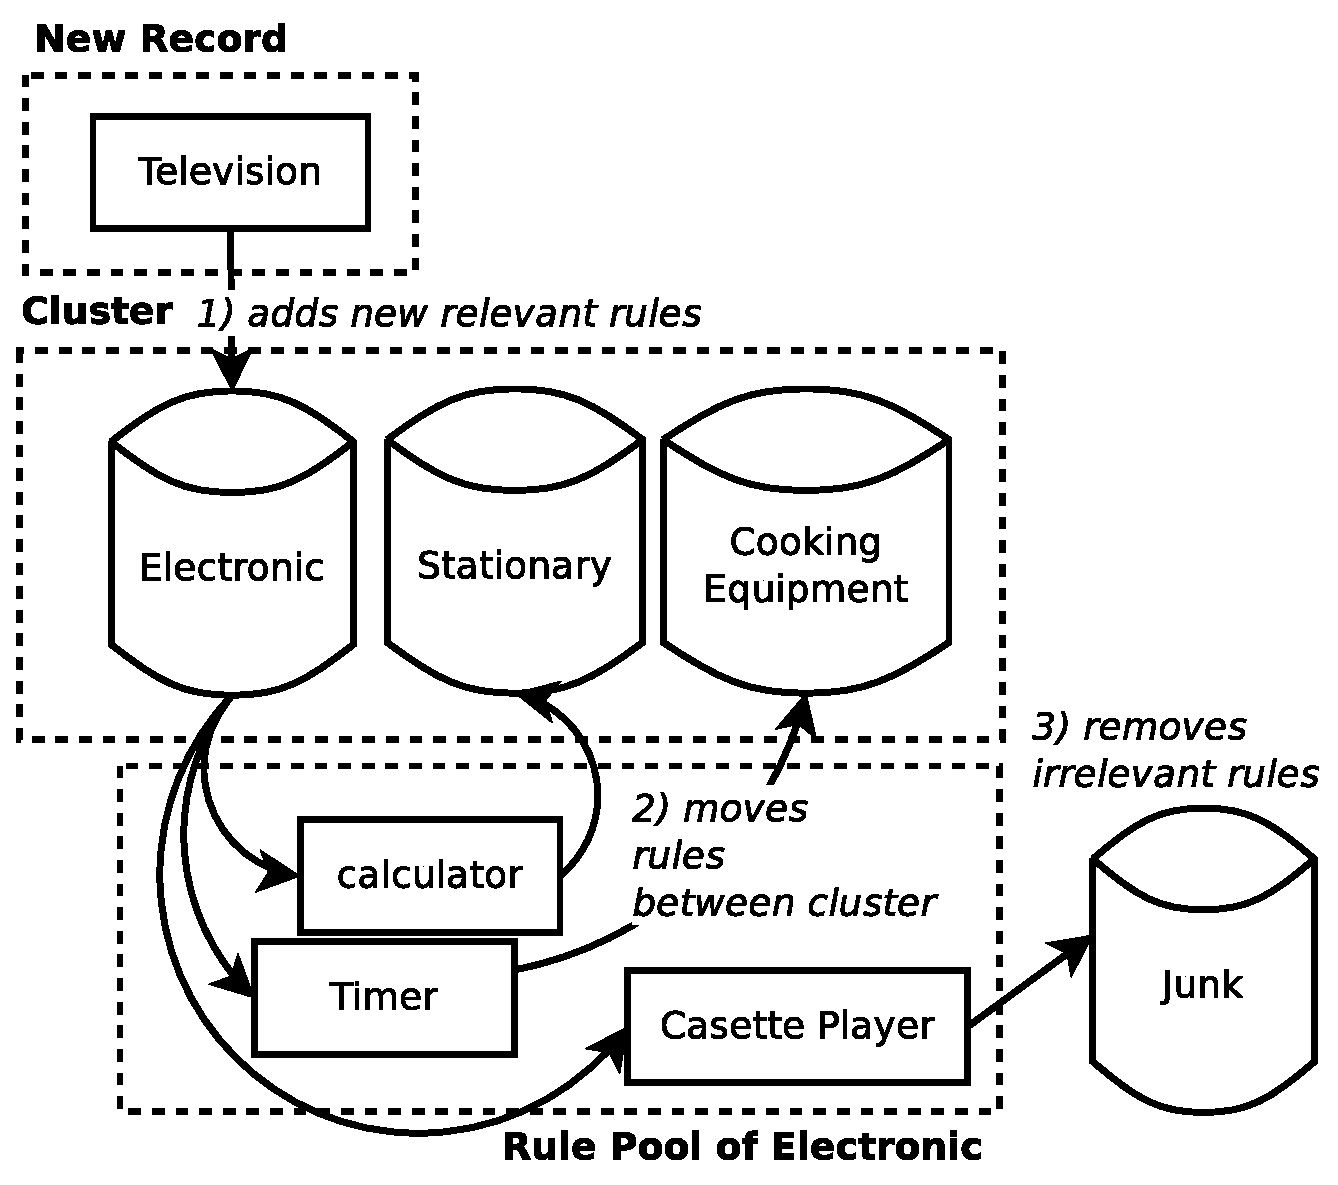
\includegraphics[width=0.3\textwidth]{mainpic}
  \end{center}
\end{wrapfigure}

Research proposed decision support of database clusters optimization using genetic network programming (GNP) with on-line rule based clustering. GNP optimize cluster quality by reanalyze weak point of each cluster and maintain rules definition that stored on each cluster. Maintenance of rules definition includes : 1) adds new relevant rules, 2) moves rules between cluster and 3) removes irrelevant rules. Research simulation focused to optimize cluster quality response against several data unbalanced data growth to the dataset that already mapped with storage rules. Simulation results of proposed method shows better result and much lower iteration time compared to GNP rule based clustering without on-line optimization.

\end{document} 